\scanpage{29}
% L1–3
\uline{Dém} Soit \inserted{pour $K\subset\Delta_n$,} $G_K=$ ss-gpe de $G$ engendré par $\{\sigma_i\mid i\in K\}$. Soit \deleted{$K=\complement_{\inserted{\Delta_n}}H,\ K'=\complement H'$} $K=\Delta_n\setminus H,\ K'=\Delta_n\setminus H'$, donc $K\cup K'=\Delta_n-H\cap H'$, la \deleted{diagramme} \inserted{flèche} envisagée est
% L4–5
\diagram{\begin{tikzcd}[ampersand replacement=\&]
X/G_{K\cap K'}\arrow[r,"p"] \& X/G_K\mathbin{\times}_{X/G_{K\cup K'}}X/G_{K'}\\
X\arrow[u]\arrow[ur,"p'"] \&
\end{tikzcd}}
% L6–8
Il suffit de prouver que $p'$ est surjectif. Je dis que l'on a
\[
G_{K\cup K'}=G_K\cdot G_{K'}
\]
(d'où \deleted{\unsure{l'énoncé|l'assertion}} le résultat s'ensuit aussitôt).
% L9–11
Or \deleted{\unsure{soit}} \inserted{soit} $i$ le dernier él. \deleted{de $K$}, \inserted{de $H$ \deleted{\unsure{donc}} de $H\cap H'$} \deleted{\unsure{Il vient}} $i\in H\cap H'$ \deleted{donc $K_0=K\cap[0,i-1]\subsetK'$} $i\notin K\cup K'$, donc
% L12 left
\margin{OPS $H\cap H'\ne H,H'$}
% L12–13
\[
\begin{aligned}
K\cup K'&=(K\cup K')\cap\underbrace{\complement\{i\}}_{[0,i-1]\amalg[i+1,n]}\\
&=\overbrace{(K\cup K')\cap[0,i-1]}^{K'_0}\\
&\quad\amalg\underbrace{(K\cup K')\cap[i+1,n]}_{K_0}
\end{aligned}
\]
% L14–15
Le dernier sommande est $\deleted{\unsure{\subset}}\subset K$ car $[i+1,n]\subset K$, le premier est $\subset K'$, car pour les $j\leq i-1$,
% L16–17 left
\figure{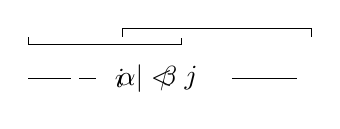
\begin{tikzpicture}[x=.75cm,y=.47cm]
\draw (0,1.1)--(0,0.9)--(2.6,.9)--(2.6,1.08);
\draw (1.6,1.12)--(1.6,1.35)--(4.8,1.35)--(4.8,1.12);
\draw (0,0)--(.72,0) (.86,0)--(1.14,0) (3.45,0)--(4.55,0);
\node at (1.55,0){$i$};\node at (1.98,0){$\unsure{\alpha|<}$};
\node at (2.38,0){$\beta$};\node at (2.76,0){$j$};
\end{tikzpicture}}
% slanted
\margin{On a utilisé a) le dernier él. de $H$ est dans $H'$ b) $H\cap H'$ est un segment initial de $H'$}
% L16–20
\deleted{\unsure{ou bien} $j\in$} Si $j\notin H\cap H'$ (i-e. $j\in K\cup K'$) \deleted{ou bien} \inserted{on a} $j\notin H'$ \deleted{(sinon}, car $H\cap H'$ est segment initial de $H'$, d'extrémité $i$, donc si $j\in H'$, on aurait $j\in H$ donc $j\in H\cap H$) donc $j\unsure{\in|\notin}H'$.
% L21–23
\deleted{Donc $G_{K\cup K'}\subset G_KG_{K'}$, d'où ég} \deleted{\unsure{Or} $G$}
Or $G_{K_0}$ et $G_{K'_0}$ \uline{commutent} donc
\[
G_{K\cup K'}\subset\underbrace{G_{K_0}\cdot G_{K'_0}}_{\text{ss-gpe}}\ \unsure{\subset|\subseteq}\ G_K\cdot G_{K'}\quad\text{cqfd.}
\]
% archive sheet number: 28
